\documentclass{standalone}
\usepackage{tikz}
\usetikzlibrary{patterns, positioning}


\begin{document}
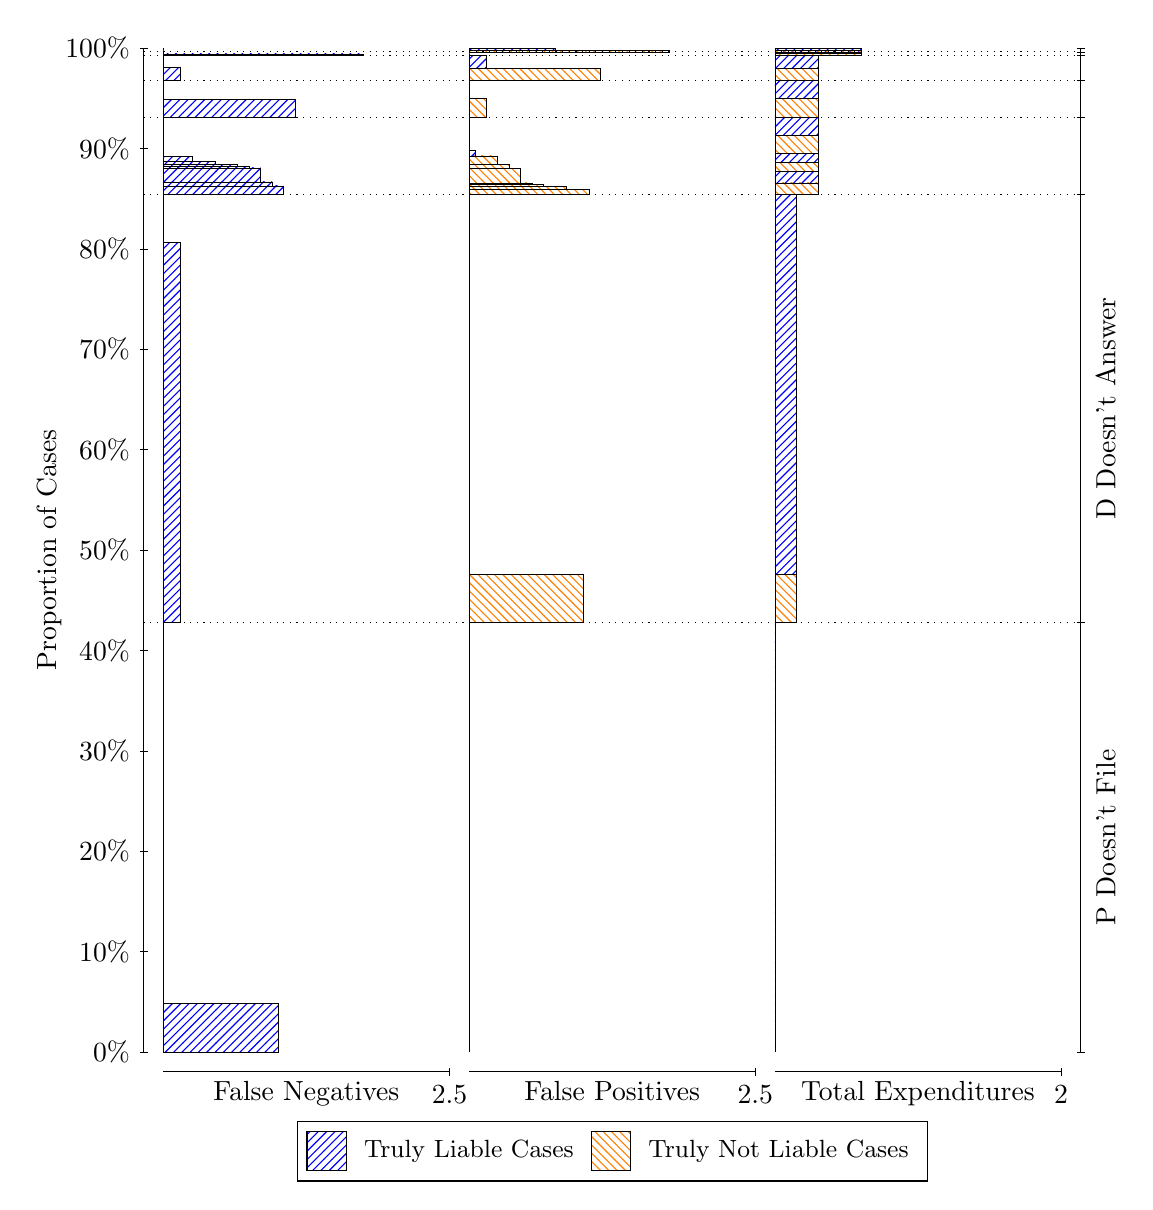
\begin{tikzpicture}
\draw[black, very thin] (1.5,1.75) -- (1.5,14.5);
\node[rotate=90, text=black, anchor=center] at (0.3, 8.125) {Proportion of Cases};
\draw[black, very thin] (1.45,1.75) -- (1.55,1.75);
\node[text=black, anchor=east] at (1.45, 1.75) {0\%};
\draw[black, very thin] (1.45,3.025) -- (1.55,3.025);
\node[text=black, anchor=east] at (1.45, 3.025) {10\%};
\draw[black, very thin] (1.45,4.3) -- (1.55,4.3);
\node[text=black, anchor=east] at (1.45, 4.3) {20\%};
\draw[black, very thin] (1.45,5.575) -- (1.55,5.575);
\node[text=black, anchor=east] at (1.45, 5.575) {30\%};
\draw[black, very thin] (1.45,6.85) -- (1.55,6.85);
\node[text=black, anchor=east] at (1.45, 6.85) {40\%};
\draw[black, very thin] (1.45,8.125) -- (1.55,8.125);
\node[text=black, anchor=east] at (1.45, 8.125) {50\%};
\draw[black, very thin] (1.45,9.4) -- (1.55,9.4);
\node[text=black, anchor=east] at (1.45, 9.4) {60\%};
\draw[black, very thin] (1.45,10.675) -- (1.55,10.675);
\node[text=black, anchor=east] at (1.45, 10.675) {70\%};
\draw[black, very thin] (1.45,11.95) -- (1.55,11.95);
\node[text=black, anchor=east] at (1.45, 11.95) {80\%};
\draw[black, very thin] (1.45,13.225) -- (1.55,13.225);
\node[text=black, anchor=east] at (1.45, 13.225) {90\%};
\draw[black, very thin] (1.45,14.5) -- (1.55,14.5);
\node[text=black, anchor=east] at (1.45, 14.5) {100\%};

\draw[black, very thin] (13.4,1.75) -- (13.4,14.5);
\draw[black, very thin] (13.35,1.75) -- (13.45,1.75);
\node[anchor=west] at (13.35, 1.75) {};
\draw[black, very thin] (13.35,7.2033) -- (13.45,7.2033);
\node[anchor=west] at (13.35, 7.2033) {};
\draw[black, very thin] (13.35,12.641) -- (13.45,12.641);
\node[anchor=west] at (13.35, 12.641) {};
\draw[black, very thin] (13.35,13.619) -- (13.45,13.619);
\node[anchor=west] at (13.35, 13.619) {};
\draw[black, very thin] (13.35,14.092) -- (13.45,14.092);
\node[anchor=west] at (13.35, 14.092) {};
\draw[black, very thin] (13.35,14.407) -- (13.45,14.407);
\node[anchor=west] at (13.35, 14.407) {};
\draw[black, very thin] (13.35,14.451) -- (13.45,14.451);
\node[anchor=west] at (13.35, 14.451) {};
\draw[black, very thin] (13.35,14.5) -- (13.45,14.5);
\node[anchor=west] at (13.35, 14.5) {};

\draw[black, very thin, pattern color=blue, pattern=north east lines] (1.75,1.75) rectangle (3.2033,2.367);
\draw[black, very thin, pattern color=orange, pattern=north west lines] (1.75,2.367) rectangle (1.75,7.2033);
\draw[black, very thin, pattern color=blue, pattern=north east lines] (1.75,7.2033) rectangle (1.968,12.032);
\draw[black, very thin, pattern color=orange, pattern=north west lines] (1.75,12.032) rectangle (1.75,12.641);
\draw[black, very thin, pattern color=blue, pattern=north east lines] (1.75,12.641) rectangle (3.276,12.749);
\draw[black, very thin, pattern color=blue, pattern=north east lines] (1.75,12.749) rectangle (3.1307,12.799);
\draw[black, very thin, pattern color=blue, pattern=north east lines] (1.75,12.799) rectangle (2.9853,12.978);
\draw[black, very thin, pattern color=blue, pattern=north east lines] (1.75,12.978) rectangle (2.84,12.997);
\draw[black, very thin, pattern color=blue, pattern=north east lines] (1.75,12.997) rectangle (2.6947,13.021);
\draw[black, very thin, pattern color=blue, pattern=north east lines] (1.75,13.021) rectangle (2.404,13.06);
\draw[black, very thin, pattern color=blue, pattern=north east lines] (1.75,13.06) rectangle (2.1133,13.128);
\draw[black, very thin, pattern color=orange, pattern=north west lines] (1.75,13.128) rectangle (1.75,13.619);
\draw[black, very thin, pattern color=blue, pattern=north east lines] (1.75,13.619) rectangle (3.4213,13.845);
\draw[black, very thin, pattern color=orange, pattern=north west lines] (1.75,13.845) rectangle (1.75,14.092);
\draw[black, very thin, pattern color=blue, pattern=north east lines] (1.75,14.092) rectangle (1.968,14.259);
\draw[black, very thin, pattern color=orange, pattern=north west lines] (1.75,14.259) rectangle (1.75,14.407);
\draw[black, very thin, pattern color=blue, pattern=north east lines] (1.75,14.407) rectangle (4.2933,14.426);
\draw[black, very thin, pattern color=orange, pattern=north west lines] (1.75,14.426) rectangle (1.75,14.451);
\draw[black, very thin, pattern color=orange, pattern=north west lines] (1.75,14.451) rectangle (1.75,14.47);
\draw[black, very thin, pattern color=blue, pattern=north east lines] (1.75,14.47) rectangle (1.75,14.5);
\draw[black, very thin, pattern color=orange, pattern=north west lines] (5.6333,1.75) rectangle (5.6333,6.5862);
\draw[black, very thin, pattern color=blue, pattern=north east lines] (5.6333,6.5862) rectangle (5.6333,7.2033);
\draw[black, very thin, pattern color=orange, pattern=north west lines] (5.6333,7.2033) rectangle (7.0867,7.8127);
\draw[black, very thin, pattern color=blue, pattern=north east lines] (5.6333,7.8127) rectangle (5.6333,12.641);
\draw[black, very thin, pattern color=orange, pattern=north west lines] (5.6333,12.641) rectangle (7.1593,12.707);
\draw[black, very thin, pattern color=orange, pattern=north west lines] (5.6333,12.707) rectangle (6.8687,12.745);
\draw[black, very thin, pattern color=orange, pattern=north west lines] (5.6333,12.745) rectangle (6.578,12.77);
\draw[black, very thin, pattern color=orange, pattern=north west lines] (5.6333,12.77) rectangle (6.4327,12.788);
\draw[black, very thin, pattern color=orange, pattern=north west lines] (5.6333,12.788) rectangle (6.2873,12.968);
\draw[black, very thin, pattern color=orange, pattern=north west lines] (5.6333,12.968) rectangle (6.142,13.018);
\draw[black, very thin, pattern color=orange, pattern=north west lines] (5.6333,13.018) rectangle (5.9967,13.131);
\draw[black, very thin, pattern color=blue, pattern=north east lines] (5.6333,13.131) rectangle (5.706,13.2);
\draw[black, very thin, pattern color=blue, pattern=north east lines] (5.6333,13.2) rectangle (5.6333,13.619);
\draw[black, very thin, pattern color=orange, pattern=north west lines] (5.6333,13.619) rectangle (5.8513,13.865);
\draw[black, very thin, pattern color=blue, pattern=north east lines] (5.6333,13.865) rectangle (5.6333,14.092);
\draw[black, very thin, pattern color=orange, pattern=north west lines] (5.6333,14.092) rectangle (7.3047,14.24);
\draw[black, very thin, pattern color=blue, pattern=north east lines] (5.6333,14.24) rectangle (5.8513,14.407);
\draw[black, very thin, pattern color=orange, pattern=north west lines] (5.6333,14.407) rectangle (5.6333,14.432);
\draw[black, very thin, pattern color=blue, pattern=north east lines] (5.6333,14.432) rectangle (5.6333,14.451);
\draw[black, very thin, pattern color=orange, pattern=north west lines] (5.6333,14.451) rectangle (8.1767,14.47);
\draw[black, very thin, pattern color=blue, pattern=north east lines] (5.6333,14.47) rectangle (6.7233,14.5);
\draw[black, very thin, pattern color=orange, pattern=north west lines] (9.5167,1.75) rectangle (9.5167,6.5862);
\draw[black, very thin, pattern color=blue, pattern=north east lines] (9.5167,6.5862) rectangle (9.5167,7.2033);
\draw[black, very thin, pattern color=orange, pattern=north west lines] (9.5167,7.2033) rectangle (9.7892,7.8127);
\draw[black, very thin, pattern color=blue, pattern=north east lines] (9.5167,7.8127) rectangle (9.7892,12.641);
\draw[black, very thin, pattern color=orange, pattern=north west lines] (9.5167,12.641) rectangle (10.062,12.788);
\draw[black, very thin, pattern color=blue, pattern=north east lines] (9.5167,12.788) rectangle (10.062,12.938);
\draw[black, very thin, pattern color=orange, pattern=north west lines] (9.5167,12.938) rectangle (10.062,13.052);
\draw[black, very thin, pattern color=blue, pattern=north east lines] (9.5167,13.052) rectangle (10.062,13.16);
\draw[black, very thin, pattern color=orange, pattern=north west lines] (9.5167,13.16) rectangle (10.062,13.389);
\draw[black, very thin, pattern color=blue, pattern=north east lines] (9.5167,13.389) rectangle (10.062,13.619);
\draw[black, very thin, pattern color=orange, pattern=north west lines] (9.5167,13.619) rectangle (10.062,13.865);
\draw[black, very thin, pattern color=blue, pattern=north east lines] (9.5167,13.865) rectangle (10.062,14.092);
\draw[black, very thin, pattern color=orange, pattern=north west lines] (9.5167,14.092) rectangle (10.062,14.24);
\draw[black, very thin, pattern color=blue, pattern=north east lines] (9.5167,14.24) rectangle (10.062,14.407);
\draw[black, very thin, pattern color=orange, pattern=north west lines] (9.5167,14.407) rectangle (10.607,14.432);
\draw[black, very thin, pattern color=blue, pattern=north east lines] (9.5167,14.432) rectangle (10.607,14.451);
\draw[black, very thin, pattern color=orange, pattern=north west lines] (9.5167,14.451) rectangle (10.607,14.47);
\draw[black, very thin, pattern color=blue, pattern=north east lines] (9.5167,14.47) rectangle (10.607,14.5);
\draw[black, dotted] (1.5,7.2033) -- (13.4,7.2033);
\draw[black, dotted] (1.5,12.641) -- (13.4,12.641);
\draw[black, dotted] (1.5,13.619) -- (13.4,13.619);
\draw[black, dotted] (1.5,14.092) -- (13.4,14.092);
\draw[black, dotted] (1.5,14.407) -- (13.4,14.407);
\draw[black, dotted] (1.5,14.451) -- (13.4,14.451);
\draw[black, very thin] (1.75,1.5) -- (5.3833,1.5);
\node[text=black, anchor=north] at (3.5667, 1.5) {False Negatives};
\draw[black, very thin] (5.3833,1.45) -- (5.3833,1.55);
\node[text=black, anchor=north] at (5.3833, 1.45) {2.5};

\draw[black, very thin] (5.6333,1.5) -- (9.2667,1.5);
\node[text=black, anchor=north] at (7.45, 1.5) {False Positives};
\draw[black, very thin] (9.2667,1.45) -- (9.2667,1.55);
\node[text=black, anchor=north] at (9.2667, 1.45) {2.5};

\draw[black, very thin] (9.5167,1.5) -- (13.15,1.5);
\node[text=black, anchor=north] at (11.333, 1.5) {Total Expenditures};
\draw[black, very thin] (13.15,1.45) -- (13.15,1.55);
\node[text=black, anchor=north] at (13.15, 1.45) {2};

\node[text=black, centered, rotate=90] at (13.72, 4.4766) {P Doesn't File};
\node[text=black, centered, rotate=90] at (13.72, 9.9223) {D Doesn't Answer};






\draw (7.449999999999999,1.5) node[draw=none] (baseCoordinate) {};
\begin{scope}[align=center]
        \matrix[scale=0.5, draw=black, below=0.5cm of baseCoordinate, nodes={draw}, column sep=0.1cm]{
            \node[rectangle, draw, minimum width=0.5cm, minimum height=0.5cm, pattern color=blue, pattern=north east lines] {}; &
            \node[draw=none, font=\small, text=black] (B) {Truly Liable Cases}; &
            \node[rectangle, draw, minimum width=0.5cm, minimum height=0.5cm, pattern color=orange, pattern=north west lines] {}; &
            \node[draw=none, font=\small, text=black] (B) {Truly Not Liable Cases}; \\
            };
\end{scope}

\end{tikzpicture}
\end{document}